\documentclass[tikz]{standalone}
\usepackage{pgffor}

\begin{document}
    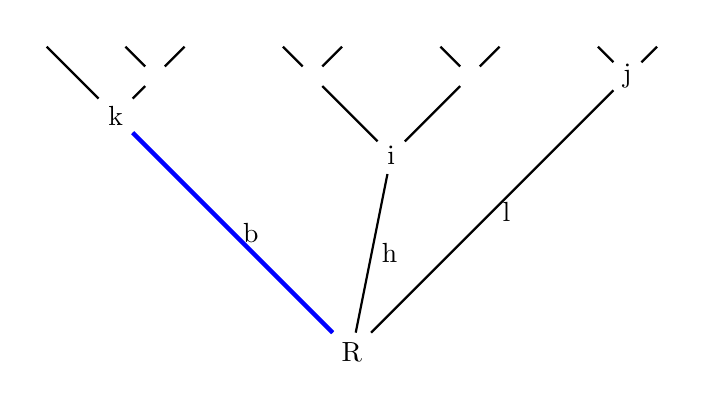
\begin{tikzpicture}
        \foreach \x/\y/\n/\l in {0/4/a/,1/4/b/,2/4/c/,3/4/d/,4/4/e/,5/4/f/,6/4/g/,7/4/h/,8/4/i/}{
            \node[] (\n) at (\x,\y) {\l};
        }
        \foreach \x/\y/\n/\l in {1.5/0.5/lnode1/,1/1/lnode2/k,3.5/0.5/k1/,5.5/0.5/k2/,4.5/1.5/k/i,7.5/0.5/rnode1/j,4/4/root/R}{
            \node[] (\n) at (\x,4-\y) {\l};
        }
        \foreach \m/\n/\l in {a/lnode2/,b/lnode1/,c/lnode1/,lnode1/lnode2/,d/k1/,e/k1/,f/k2/,g/k2/,k1/k/,k2/k/,h/rnode1/,i/rnode1/,k/root/h,rnode1/root/l,lnode2/root/b}{
            \draw[thick] (\m) -- node[right]{\l} (\n);
        }
        \draw[ultra thick, blue] (lnode2) -- (root);
    \end{tikzpicture}
\end{document}